
\chapter*{Quantum computers and mapping of quantum circuits}
\label{sec:org3eae870}

\section*{Quantum computing}
\label{sec:orga07d5c7}

[Intro to Quantum Computation power that it is based on \textbf{superposition} and *entanglement*]
In this section \ldots{}

\subsection*{Essential elements of quantum computation}
\label{sec:org1512db5}

Qubits and quantum gates are the basic ingredients in quantum computation theory.
As in classical computation with boolean gates and bits, quantum gates operate on the qubits to change their state and return the desired result or calculation.

\begin{itemize}
\item Qubits
\label{sec:org4d0baab}

Qubit stands for quantum bit.
A basic unit of information founded on quantum physics laws.
Unlike a classical bit, whose state can be either \texttt{0} or \texttt{1}, but like a particle; qubits are not in a fixed state -- ground or excited -- until they are measured.
A qubit's state could be either \texttt{0} or \texttt{1} or both before measuring it.
Both ground or excited states are represented in the Dirac's bra-ket notation, viz. \(| 0 \rangle\) and \(| 1 \rangle\) respectively.
This notation holds the algebraic axioms \cite{Nielsen_2009} required to understand the quantum theory.
Prior to measurement, a qubit is described as in a probabilistic state \(| \psi \rangle = \alpha | 0 \rangle + \beta | 1 \rangle\), where \(\alpha, \beta \in \mathbb{C}\) are the so-called probability amplitudes.
\(|\alpha|^2\) is the probability of measuring \(| 0 \rangle\), \(|\beta|^2\) is the probability of measuring \(| 1 \rangle\) and both \(\alpha\) and \(\beta\) are allowed to be complex.
Dirac's notation grants the definition of the quantum states as vectors, as in eq. \ref{eq:orgde6efa2}.
Moreover, as we will see below, adopting Dirac's axioms will make the quantum theory accessible with classical algebra operations. 

\begin{equation}
\label{eq:orgde6efa2}
|\psi\rangle = \begin{bmatrix}\alpha \\ \beta \end{bmatrix}
\end{equation}

\textbf{Superposition} is easily described giving values to both \(\alpha\) and \(\beta\) in the same vector.
But, as soon as they are energy probabilistic states, their values are constrained to \(|\alpha|^2 + |\beta|^2 = 1\).
Since quantum states can be described as vectors, one can easily see that the state of a qubit is defined by a 2-dimensional, complex and unitarian vector space.
A \textbf{Hilbert space} \(\mathscr{H}\).
E.g. in eq. \ref{eq:org8ae880c} the vectors of the ground, excited and the plus superposition -- a quantum state with the same probability to measure either \(|0\rangle\) or \(|1\rangle\) -- states are depicted, respectively.

\begin{equation}
\label{eq:org8ae880c}
|0\rangle = \begin{bmatrix}1 \\ 0 \end{bmatrix} \quad \quad |1\rangle = \begin{bmatrix}0 \\ 1 \end{bmatrix} \quad \quad |+\rangle = \frac{1}{\sqrt{2}} \begin{bmatrix}1 \\ 1 \end{bmatrix}
\end{equation}

As soon as the vectors are 2-dimensional, complex and unitary they can also be described in phase notation (eq. \ref{eq:orgaec79b9}).
Like the complex numbers, although requiring two angles in this case.
This notation lead us to a very understandable way to visualize the quantum states, the \textbf{Bloch sphere} (fig. \ref{fig:bloch_sphere}).
A sphere of radius one which z-axis extremes represent the ground and excited states.

\begin{equation}
\label{eq:orgaec79b9}
|\psi \rangle =\cos \left(\theta /2\right)|0\rangle \,+\,e^{i\phi }\sin \left(\theta /2\right)|1\rangle
\end{equation}

\begin{figure}
\centering
\begin{tikzpicture}[line cap=round, line join=round, >=Triangle]
  \clip(-2.19,-2.49) rectangle (2.66,2.58);
  \draw [shift={(0,0)}, lightgray, fill, fill opacity=0.1] (0,0) -- (56.7:0.4) arc (56.7:90.:0.4) -- cycle;
  \draw [shift={(0,0)}, lightgray, fill, fill opacity=0.1] (0,0) -- (-135.7:0.4) arc (-135.7:-33.2:0.4) -- cycle;
  \draw(0,0) circle (2cm);
  \draw [rotate around={0.:(0.,0.)},dash pattern=on 3pt off 3pt] (0,0) ellipse (2cm and 0.9cm);
  \draw (0,0)-- (0.70,1.07);
  \draw [->] (0,0) -- (0,2);
  \draw [->] (0,0) -- (-0.81,-0.79);
  \draw [->] (0,0) -- (2,0);
  \draw [dotted] (0.7,1)-- (0.7,-0.46);
  \draw [dotted] (0,0)-- (0.7,-0.46);
  \draw (-0.08,-0.3) node[anchor=north west] {$\varphi$};
  \draw (0.01,0.9) node[anchor=north west] {$\theta$};
  \draw (-1.01,-0.72) node[anchor=north west] {$\mathbf {\hat{x}}$};
  \draw (2.07,0.3) node[anchor=north west] {$\mathbf {\hat{y}}$};
  \draw (-0.5,2.6) node[anchor=north west] {$\mathbf {\hat{z}=|0\rangle}$};
  \draw (-0.4,-2) node[anchor=north west] {$-\mathbf {\hat{z}=|1\rangle}$};
  \draw (0.4,1.65) node[anchor=north west] {$|\psi\rangle$};
  \scriptsize
  \draw [fill] (0,0) circle (1.5pt);
  \draw [fill] (0.7,1.1) circle (0.5pt);
\end{tikzpicture}
\caption{The Bloch sphere}
\label{fig:bloch_sphere}
\end{figure}

But a system with just one qubit is not useful.
The power of quantum computers explodes with the number of qubits able to work with or, what is the same, the dimensions of the Hilbert space \(\mathscr{H}\).
The quantum state of \(n\) qubits can be represented in bra-ket notation, with a \(2^n\) size.
And, therefore, they engender a Hilbert space of \(2^n\) dimensions due to superposition.
The linear operator that leads to the multiple qubit's state is the \textbf{outer product}, defined as the matrix convolution of the state vectors.
The outer product is represented as \(|\phi \rangle \,\langle \psi |\).
In eq. \ref{eq:orge9f6cbe} and \ref{eq:org7b15f84} an example of the outer product is offered.
The second example represents the other main phenomenon in quantum physics, the \textbf{entanglement} state of two qubits (\(\phi\) and \(\psi\)) also known as the Bell state or the Einstein-Podolsky-Rosen (EPR) pair.

\begin{equation}
\label{eq:orge9f6cbe}
|+\rangle \,\langle + | = \frac{1}{\sqrt{4}} \left( \begin{bmatrix}1 \\ 1 \end{bmatrix} \otimes \begin{bmatrix}1 \\ 1 \end{bmatrix} \right) = \frac{1}{\sqrt{4}} \begin{bmatrix}1 \\ 1 \\ 1 \\ 1\end{bmatrix} 
\end{equation}

\begin{equation}
\label{eq:org7b15f84}
|\Phi ^{+}\rangle =\frac  {1}{\sqrt  {2}}(|0\rangle _{\phi}\otimes |0\rangle _{\psi}+|1\rangle _{\phi}\otimes |1\rangle _{\psi}) =  \frac{(|00\rangle +|11\rangle )} {\sqrt {2}}
\end{equation}


\item Quantum Operations
\label{sec:org04e65ed}

Quantum operations leverage the power of quantum computers enabling calculations over the qubits.
Or what is the same, enabling transformations of a Hilbert space.
One can find a parallelism with the classical computation fundamental operations, the logical operations.
As their classical siblings, the quantum operations are usually represented as gates in a circuit, a so-called quantum circuit.
Quantum operations can be described in Dirac's notation as well.
They are represented as square matrices of \(2^{n} \times 2^{n}\), where \(n\) is the number of qubits involved in the operation.
This matrices should be unitary respecting the qubit state vector unitary property (\(|\alpha|^2 + |\beta|^2 = 1\)).
They shouldn't ever change the amplitude of the state.
Therefore, quantum operations are, basically, state rotations in the Bloch sphere (fig. \ref{fig:bloch_sphere}).
Although, while implying multiple qubits, the quantum operations are more complex than just rotations, as it will be seen below.
For instance, a rotation of 180° in z-axis of the Bloch sphere is the same as an operation that change the qubit state from \(| 0 \rangle\) to \(| 1 \rangle\), or viceversa.
Qubits and quantum operations interact through the \textbf{inner product}.
In order to apply some operation over a qubit state, a matrix-vector multiplication should be done.
For instance, in eq. \ref{eq:orgc99bb6d} one can understand how some uniform operation \(U\) is applied to a qubit with state \(| \psi \rangle\).

\begin{equation}
\label{eq:orgc99bb6d}
U |\psi\rangle=\begin{bmatrix}u_{00}&u_{01}\\u_{10}&u_{11}\end{bmatrix} \begin{bmatrix}\alpha \\ \beta \end{bmatrix} = \begin{bmatrix}\alpha u_{00} + \beta u_{01} \\ \alpha u_{10} + \beta u_{11} \end{bmatrix}
\end{equation}

Also comparable with the boolean gates, quantum operations can be decomposed in other set of quantum operations.
\textbf{Universal set of gates} is a set of operations able to generate any other gate by combining them \cite{Nielsen_2009}.
In classical computation, for example, the \texttt{OR} and the \texttt{AND} gates are able to generate any other logic gate.
In quantum computation there are several universal set of gates.
In the \href{chapter-3.org}{Constraints of the Surface-7 and -17 chips} section we offer a table with a universal gate set with its decomposition, particularized for the SC-7 and -17 chips which specifications will be also described in that section.
It is common to differ between single- and multiple-qubit gates, due to the complexity variation between them.
It is generally accepted to analyze the multiple-qubit gate problem in its most elemental case, that is the two-qubit gates.

\begin{itemize}
\item Single-qubit gates
\label{sec:org047c88b}

Single qubit gates represent quantum operations that involve just one qubit.
They are represented as a box with one input and one output, evincing that a single qubit will be the input and output of the operation.
As explained before, single-qubit gates can be represented as \(2^1 \times 2^1\) square matrices that should be unitary.
Both representations of the most common single-qubit gates can be found in the table \ref{tab:single_q_gates}.

\begin{table}[htbp]
\caption{\label{tab:org170590e}
Most common single qubit gates}
\centering
\begin{tabular}{c}
Pauli-X\\
\Qcircuit @C=1em @R=.7em {
  \lstick{\shortmid q\rangle} & \gate{I} & \qw\\
}
\\
\end{tabular}
\end{table}

\item Two-qubit gates
\label{sec:orgd273516}
The most common two-qubit gates are 
As the single-qubit gates, two qubit gates
\end{itemize}
\end{itemize}


\subsection*{Quantum Circuits}
\label{sec:orga42a1df}

Quantum circuits are quantum algorithms descriptions.
As mentioned before, they are formed by quantum gates and qubits connected in circuit fashion.
As most of the algorithm description models, quantum circuits are hardware agnostic, which is that they are not specified to any quantum device.
They are general descriptions of quantum algorithms.
Besides the circuit description model, quantum algorithms are commonly described as instruction languages like QASM (Quantum ASseMbly) \cite{Nielsen_2009} or its related posterior languages -- cQASM, OpenQASM, \ldots{}
In fig. \ref{fig:circuit_example} we present an example of a quantum circuit.
This circuit represents the quantum equivalent of a Gray encoder of six bit length.
It is composed by CNOT gates only.
An example of the Gray code is shown in \ref{fig:org619522d} for different number of bits (\(n\)).
Also, the QASM algorithm representation can be seen in code \ref{org6c3c4ee}.

\begin{figure}
    \centering

\resizebox{0.3\textwidth}{!}{
   \Qcircuit @C=1em @R=.7em {
\lstick{a} & \targ & \qw & \qw & \qw & \qw & \qw\\
\lstick{b} & \ctrl{-1} & \targ & \qw & \qw & \qw & \qw\\
\lstick{c} & \qw & \ctrl{-1} & \targ & \qw & \qw & \qw\\
\lstick{d} & \qw & \qw & \ctrl{-1} & \targ & \qw & \qw\\
\lstick{e} & \qw & \qw & \qw & \ctrl{-1} & \targ & \qw\\
\lstick{f} & \qw & \qw & \qw & \qw & \ctrl{-1} & \qw
}
}

\label{fig:circuit_example}
\caption{Gray encoder quantum circuit.}
\end{figure}

\begin{figure}[htbp]
\centering
\includegraphics[width=0.3\textwidth]{figures/gray_code.png}
\caption{\label{fig:org619522d}
Gray Code example for 3 bits.}
\end{figure}

\begin{figure}
\centering
\begin{minipage}{.45\textwidth}

\begin{minted}[frame=lines,fontsize=\scriptsize,linenos,breaklines,breakanywhere]{c}

#QASM code

# qubit declaration
qubit a
qubit b
qubit c
qubit d
qubit e
qubit f

# gates declaration
cnot b,a
cnot c,b
cnot d,c
cnot e,d
cnot f,d

\end{minted}

\caption{QASM code describing the Gray code algorithm.}
\end{minipage}
\end{figure}

\section*{Mapping of quantum circuits}
\label{sec:org27a23c8}

\subsection*{Mapping}
\label{sec:org14614d9}

Given a quantum circuit representation that is hardware agnostic, adapt it to the requirements of a real quantum processor.


The mapping problem can be split in:

\begin{itemize}
\item Scheduling
\item Placement
\item Routing
\end{itemize}

\begin{itemize}
\item {\bfseries\sffamily TODO} :B\(_{\text{noteNH}}\):
\label{sec:orge854428}
So, what is mapping?
Given a quantum circuit representation that is hardware agnostic, the mapping task adapt it to the requirements of a real quantum processor.

The mapping problem can be split in 3 parts that are executed continuously:

\begin{itemize}
\item Scheduling. How is better to organize the operation in the quantum circuit along time?
\item Placement. What is the best way to initialize the qubits?
\item Routing. What is the best way for moving the information between qubits?
\end{itemize}
\end{itemize}

\subsection*{Scheduling}
\label{sec:orgae9b5c4}

\begin{itemize}
\item Example
\label{sec:orgdf9e0f0}
\begin{itemize}
\item Original
\label{sec:org6d9e2e4}

\begin{center}

Original

   \Qcircuit @C=1em @R=.7em {
 & \qswap & \qw & \gate{X} & \qw & \qw\\
 & \qw & \ctrl{2} & \qw & \qw & \qw\\
 & \qswap \qwx[-2] & \qw & \qw & \gate{H} & \qw\\
 & \qw & \targ & \qw & \qw & \qw\\
}
\end{center}

\item ASAP
\label{sec:orge6ac5e9}

\begin{center}

ASAP

   \Qcircuit @C=1em @R=.7em {
 &  &  & \qwx[5] &  & \\
 & \qswap & \qw & \qw & \gate{X} & \qw\\
 & \qw & \ctrl{2} & \qw & \qw & \qw\\
 & \qswap \qwx[-2] & \qw & \qw & \gate{H} & \qw\\
 & \qw & \targ & \qw & \qw & \qw\\
 &  &  &  &  & \\
}
\end{center}

\item ALAP
\label{sec:orgb4ff0fe}

\begin{center}

ALAP

   \Qcircuit @C=1em @R=.7em {
 &  & \qwx[5] &  &  & \\
 & \qswap & \qw & \gate{X} & \qw & \qw\\
 & \qw & \qw & \ctrl{2} & \qw & \qw\\
 & \qswap \qwx[-2] & \qw & \qw & \gate{H} & \qw\\
 & \qw & \qw & \targ & \qw & \qw\\
 &  &  &  &  &  & \\
}
\end{center}
\end{itemize}

\item Dependence graph
\label{sec:org040cbb0}
\begin{itemize}
\item :BMCOL:
\label{sec:org36951a4}
The SWAP gate swaps the information between qubits.

\item Dependence graph
\label{sec:org9b2f17b}

\begin{center}
\resizebox{.5\textwidth}{!}{%
\begin{tikzpicture}
    
    \node [draw, rectangle] (a) at (0,3) {a};
    \node [draw, rectangle] (b) at (0,2) {b};
    \node [draw, rectangle] (c) at (0,1) {c};
    \node [draw, rectangle] (d) at (0,0) {d};

    
    \node [draw, ellipse] (swap) at (2,2) {SWAP};
    \node [draw, ellipse] (cnot) at (2,1) {CNOT};
    \node [draw, ellipse] (x) at (4,2.5) {X};
    \node [draw, ellipse] (h) at (4,1.5) {H};
   
    
    \draw (a) -- (swap);
    \draw (c) -- (swap);
    
    \draw (b) -- (cnot);
    \draw (d) -- (cnot);
    
    \draw (swap) -- (h);
    
    \draw (swap) -- (x);
    
    
\end{tikzpicture}
}
\end{center}

\item :BMCOL:
\label{sec:org20608f9}
Parallel operation \(\to\) the ones that can be done simultaneously
\end{itemize}

\item {\bfseries\sffamily TODO} :B\(_{\text{noteNH}}\):
\label{sec:org516ffd4}
As an example of scheduling, let's consider this circuit with\ldots{}

A SWAP gate swaps the information (or state) of one qubit to other and viceversa.

Notice that, in the example, there are several combinations of parallel operations,
or what is the same, operations that can be done simultaneously.
They don't depend on each other.

Depending on the scheduling one may want to implement,
the operations will be spread along the circuit in one way or the other.
For example, ASAP or ALAP.
\end{itemize}

\subsection*{Mapping example}
\label{sec:org2d05616}


\begin{itemize}
\item Example definition
\label{sec:orgac53be1}
\begin{itemize}
\item Example definition
\label{sec:orgecb1667}
\begin{center}

Ex.: To map the Gray code generator Quantum Circuit for 6 \uline{physical} qubits in the SC-7.

\end{center}

\item Surface architecture
\label{sec:org66e88e6}
\begin{itemize}
\item :B\(_{\text{onlyenv}}\):
\label{sec:orgf37db99}

    \begin{center}
    \resizebox{\textwidth}{!}{%
    \begin{tikzpicture}[x=5mm,y=5mm]
% \tikzstyle{every node} = [circle, fill=gray!30]
% \node [green] at (0,0) {[circle, fill=gray!30]};
\draw node[fill=cyan,circle,minimum size=0.3cm] at (0,0) {};
% \node [cyan] at (10,0) {\textbullet};
\draw node[fill=cyan,circle,minimum size=0.3cm] at (10,0) {};
% \node [green] at (20,0) {\textbullet};
\draw node[fill=cyan,circle,minimum size=0.3cm] at (20,0) {};
% \node [red] at (5,5) {\textbullet};
\draw node[fill=cyan,circle,minimum size=0.3cm] at (5,5) {};
% \node [red] at (5,-5) {\textbullet};
\draw node[fill=cyan,circle,minimum size=0.3cm] at (5,-5) {};
% \node [red] at (15,5) {\textbullet};
\draw node[fill=cyan,circle,minimum size=0.3cm] at (15,5) {};
% \node [red] at (15,-5) {\textbullet};
\draw node[fill=cyan,circle,minimum size=0.3cm] at (15,-5) {};

\node [purple] at (1,0) {\textbf{2}};
\node [purple] at (11,0) {\textbf{3}};
\node [purple] at (21,0) {\textbf{4}};
\node [purple] at (6,5) {\textbf{0}};
\node [purple] at (6,-5) {\textbf{5}};
\node [purple] at (16,5) {\textbf{1}};
\node [purple] at (16,-5) {\textbf{6}};

% \draw[{Circle[red]}-Latex] (0,0) -- (2,0);
\draw[-Latex] (0.1, 0.4)  -- (4.6,4.9)   node [midway, above, sloped] {0};
\draw[-Latex] (4.8,4.7)   -- (0.3,0.2)  node [midway, below, sloped] {8};

\draw[-Latex] (5.4, 4.9)   -- (9.9,0.4)  node [midway, above, sloped] {1};
\draw[-Latex] (9.7,0.2) -- (5.2,4.7)   node [midway, below, sloped] {9};

\draw[-Latex] (10.1,0.4)  -- (14.6,4.9)  node [midway, above, sloped] {2};
\draw[-Latex] (14.8,4.7)  -- (10.3,0.2) node [midway, below, sloped] {10};

\draw[-Latex] (15.4, 4.9)  -- (19.9,0.4)  node [midway, above, sloped] {3};
\draw[-Latex] (19.7,0.2) -- (15.2,4.7)  node [midway, below, sloped] {11};

\draw[-Latex] (0.4,-0.1) -- (4.9,-4.6)  node [midway, above, sloped] {4};
\draw[-Latex] (4.7,-4.8) -- (0.2,-0.3)  node [midway, below, sloped] {12};

\draw[-Latex] (5.1, -4.6) -- (9.6,-0.1) node [midway, above, sloped] {5};
\draw[-Latex] (9.8, -0.3) -- (5.3, -4.8) node [midway, below, sloped] {13};

\draw[-Latex] (10.4,-0.1) -- (14.9,-4.6) node [midway, above, sloped] {6};
\draw[-Latex] (14.7,-4.8) -- (10.2,-0.3) node [midway, below, sloped] {14};

\draw[-Latex] (15.1,-4.6) -- (19.6,-0.1) node [midway, above, sloped] {7};
\draw[-Latex] (19.8,-0.3)  -- (15.3,-4.8) node [midway, below, sloped] {15};

\end{tikzpicture}
}
\end{center}

\begin{center}
\resizebox{.4\textwidth}{!}{%

\begin{tikzpicture}[qubit/.style={fill=cyan,circle,minimum size=0.3cm}]

\node [qubit,label=right:Physical qubits] {Qubit};

\end{tikzpicture}
}
\end{center}



\item :B\(_{\text{onlyenv}}\):
\label{sec:org408b8d6}

    \begin{center}
    \resizebox{\textwidth}{!}{%
    \begin{tikzpicture}[x=5mm,y=5mm]
% \tikzstyle{every node} = [circle, fill=gray!30]
% \node [green] at (0,0) {[circle, fill=gray!30]};
\draw node[fill=cyan,circle,minimum size=0.3cm] at (0,0) {};
% \node [cyan] at (10,0) {\textbullet};
\draw node[fill=cyan,circle,minimum size=0.3cm] at (10,0) {};
% \node [green] at (20,0) {\textbullet};
\draw node[fill=cyan,circle,minimum size=0.3cm] at (20,0) {};
% \node [red] at (5,5) {\textbullet};
\draw node[fill=cyan,circle,minimum size=0.3cm] at (5,5) {};
% \node [red] at (5,-5) {\textbullet};
\draw node[fill=cyan,circle,minimum size=0.3cm] at (5,-5) {};
% \node [red] at (15,5) {\textbullet};
\draw node[fill=cyan,circle,minimum size=0.3cm] at (15,5) {};
% \node [red] at (15,-5) {\textbullet};
\draw node[fill=cyan,circle,minimum size=0.3cm] at (15,-5) {};

\node [purple] at (2,0) {\textbf{b} $\to$ \textbf{2}};
\node [purple] at (12,0) {\textbf{d} $\to$ \textbf{3}};
\node [purple] at (22,0) {\textbf{f} $\to$ \textbf{4}};
\node [purple] at (7,5) {\textbf{a} $\to$ \textbf{0}};
\node [purple] at (7,-5) {\textbf{c} $\to$ \textbf{5}};
\node [purple] at (17,5) {\textbf{e} $\to$ \textbf{1}};
\node [purple] at (17,-5) {\textbf{6}};

% \draw[{Circle[red]}-Latex] (0,0) -- (2,0);
\draw[-Latex] (0.1, 0.4)  -- (4.6,4.9)   node [midway, above, sloped] {0};
\draw[-Latex] (4.8,4.7)   -- (0.3,0.2)  node [midway, below, sloped] {8};

\draw[-Latex] (5.4, 4.9)   -- (9.9,0.4)  node [midway, above, sloped] {1};
\draw[-Latex] (9.7,0.2) -- (5.2,4.7)   node [midway, below, sloped] {9};

\draw[-Latex] (10.1,0.4)  -- (14.6,4.9)  node [midway, above, sloped] {2};
\draw[-Latex] (14.8,4.7)  -- (10.3,0.2) node [midway, below, sloped] {10};

\draw[-Latex] (15.4, 4.9)  -- (19.9,0.4)  node [midway, above, sloped] {3};
\draw[-Latex] (19.7,0.2) -- (15.2,4.7)  node [midway, below, sloped] {11};

\draw[-Latex] (0.4,-0.1) -- (4.9,-4.6)  node [midway, above, sloped] {4};
\draw[-Latex] (4.7,-4.8) -- (0.2,-0.3)  node [midway, below, sloped] {12};

\draw[-Latex] (5.1, -4.6) -- (9.6,-0.1) node [midway, above, sloped] {5};
\draw[-Latex] (9.8, -0.3) -- (5.3, -4.8) node [midway, below, sloped] {13};

\draw[-Latex] (10.4,-0.1) -- (14.9,-4.6) node [midway, above, sloped] {6};
\draw[-Latex] (14.7,-4.8) -- (10.2,-0.3) node [midway, below, sloped] {14};

\draw[-Latex] (15.1,-4.6) -- (19.6,-0.1) node [midway, above, sloped] {7};
\draw[-Latex] (19.8,-0.3)  -- (15.3,-4.8) node [midway, below, sloped] {15};


\end{tikzpicture}
}
\end{center}
\end{itemize}

\item :B\(_{\text{onlyenv}}\):
\label{sec:org8ae78b9}
\begin{itemize}
\item :B\(_{\text{structureenv}}\):
\label{sec:org5565816}
\begin{center}

\uline{Optimized Approach}

\medskip
\end{center}
\end{itemize}
\end{itemize}
\item :BMCOL:
\label{sec:orgf54dc40}



\item Gray Code Quantum Circuit
\label{sec:orga8af360}
\uline{Gray Code Quantum Circuit}

\begin{itemize}
\item :B\(_{\text{onlyenv}}\):
\label{sec:org2fe78a0}
\begin{verbatim}

#QASM code

qubit a
qubit b
qubit c
qubit d
qubit e
qubit f

cnot b,a
cnot c,b
cnot d,c
cnot e,d
cnot f,d

\end{verbatim}


\item :B\(_{\text{onlyenv}}\):
\label{sec:org0c39e70}

\begin{center}
   \Qcircuit @C=1em @R=.7em {
\lstick{a} & \targ & \qw & \qw & \qw & \qw & \qw\\
\lstick{b} & \ctrl{-1} & \targ & \qw & \qw & \qw & \qw\\
\lstick{c} & \qw & \ctrl{-1} & \targ & \qw & \qw & \qw\\
\lstick{d} & \qw & \qw & \ctrl{-1} & \targ & \qw & \qw\\
\lstick{e} & \qw & \qw & \qw & \ctrl{-1} & \targ & \qw\\
\lstick{f} & \qw & \qw & \qw & \qw & \ctrl{-1} & \qw
}
\end{center}


\resizebox{\textwidth}{!}{%
\begin{tikzpicture}

%maximum width= pt
    
    \node [draw, rectangle] (a) at (0,5) {a};
    \node [draw, rectangle] (b) at (0,4) {b};
    \node [draw, rectangle] (c) at (0,3) {c};
    \node [draw, rectangle] (d) at (0,2) {d};
    \node [draw, rectangle] (e) at (0,1) {e};
    \node [draw, rectangle] (f) at (0,0) {f};
    
    \node [draw, ellipse] (cnot1) at (2,4.5) {CNOT a,b};
    \node [draw, ellipse] (cnot2) at (4,3.5) {CNOT b,c};
    \node [draw, ellipse] (cnot3) at (6,2.5) {CNOT c,d};
    \node [draw, ellipse] (cnot4) at (8,1.5) {CNOT d,e};
    \node [draw, ellipse] (cnot5) at (10,0.5) {CNOT e,f};


    \draw (a) -- (cnot1);
    \draw (b) -- (cnot1);
    
    \draw (cnot1) -- (cnot2);
    \draw (c) -- (cnot2);
    
    \draw (cnot2) -- (cnot3);
    \draw (d) -- (cnot3);
    
    \draw (cnot3) -- (cnot4);
    \draw (e) -- (cnot4);
    
    \draw (cnot4) -- (cnot5);
    \draw (f) -- (cnot5);
    
\end{tikzpicture}
}

Latency: 400ns

\item :B\(_{\text{onlyenv}}\):
\label{sec:org22f77e4}
      \begin{center}
     \Qcircuit @C=1em @R=.7em {
     \lstick{a \to Q_0} & \targ & \qw & \qw & \qw & \qw & \qw\\
\lstick{b \to Q_2} & \ctrl{-1} & \targ & \qw & \qw & \qw & \qw\\
\lstick{c \to Q_5} & \qw & \ctrl{-1} & \targ & \qw & \qw & \qw\\
\lstick{d \to Q_3} & \qw & \qw & \ctrl{-1} & \targ & \qw & \qw\\
\lstick{e \to Q_1} & \qw & \qw & \qw & \ctrl{-1} & \targ & \qw\\
\lstick{f \to Q_4} & \qw & \qw & \qw & \qw & \ctrl{-1} & \qw
}
\end{center}

\tiny{* Virtual qubit $\to$ physical qubit}

Latency: 400ns
\end{itemize}

\item {\bfseries\sffamily TODO} :B\(_{\text{noteNH}}\):
\label{sec:org84b29b4}
\begin{itemize}
\item :B\(_{\text{onlyenv}}\):
\label{sec:orga5ce591}
Maybe is going to be more clear with a toy example.
Let's say that we want to run the Gray Code Quantum Generator in the SC-7.

This code is written in QASM (Quantum Assembly), a basic language for describing quantum circuits

\begin{figure}[htbp]
\centering
\includegraphics[width=0.3\textwidth]{figs/gray_code.png}
\caption{Gray Code}
\end{figure}

\item :B\(_{\text{onlyenv}}\):
\label{sec:org2ece3fb}
The Gray Code Quantum Circuit looks like this.

We have to define whish virtual qubits (a,b,\ldots{}) is related with the physical ones (0,1,..)

As you can see in the circuit and in the dependence graph there are no parallel operations, thus there is no possible scheduling.

\hline

With an optimized initial placement, or a real optimized mapping the circuit could be the  same without adding any gate.
No routing is required.
\end{itemize}
\end{itemize}

\subsection*{Mapping example. Scheduling and placement}
\label{sec:org14a5798}
\begin{itemize}
\item Example definition
\label{sec:org75e78a3}
\begin{itemize}
\item Example definition
\label{sec:org043493f}
\begin{center}

Ex.: To map the Gray code generator Quantum Circuit for 6 \uline{physical} qubits in the SC-7.

\end{center}

\item Surface architecture
\label{sec:orgb73341c}

    \begin{center}
    \resizebox{\textwidth}{!}{%
    \begin{tikzpicture}[x=5mm,y=5mm]
% \tikzstyle{every node} = [circle, fill=gray!30]
% \node [green] at (0,0) {[circle, fill=gray!30]};
\draw node[fill=cyan,circle,minimum size=0.3cm] at (0,0) {};
% \node [cyan] at (10,0) {\textbullet};
\draw node[fill=cyan,circle,minimum size=0.3cm] at (10,0) {};
% \node [green] at (20,0) {\textbullet};
\draw node[fill=cyan,circle,minimum size=0.3cm] at (20,0) {};
% \node [red] at (5,5) {\textbullet};
\draw node[fill=cyan,circle,minimum size=0.3cm] at (5,5) {};
% \node [red] at (5,-5) {\textbullet};
\draw node[fill=cyan,circle,minimum size=0.3cm] at (5,-5) {};
% \node [red] at (15,5) {\textbullet};
\draw node[fill=cyan,circle,minimum size=0.3cm] at (15,5) {};
% \node [red] at (15,-5) {\textbullet};
\draw node[fill=cyan,circle,minimum size=0.3cm] at (15,-5) {};

\node [purple] at (2,0) {\textbf{c} $\to$ \textbf{2}};
\node [purple] at (12,0) {\textbf{d} $\to$ \textbf{3}};
\node [purple] at (22,0) {\textbf{e} $\to$ \textbf{4}};
\node [purple] at (7,5) {\textbf{a} $\to$ \textbf{0}};
\node [purple] at (7,-5) {\textbf{f} $\to$ \textbf{5}};
\node [purple] at (17,5) {\textbf{b} $\to$ \textbf{1}};
\node [purple] at (17,-5) {\textbf{6}};

% \draw[{Circle[red]}-Latex] (0,0) -- (2,0);
\draw[-Latex] (0.1, 0.4)  -- (4.6,4.9)   node [midway, above, sloped] {0};
\draw[-Latex] (4.8,4.7)   -- (0.3,0.2)  node [midway, below, sloped] {8};

\draw[-Latex] (5.4, 4.9)   -- (9.9,0.4)  node [midway, above, sloped] {1};
\draw[-Latex] (9.7,0.2) -- (5.2,4.7)   node [midway, below, sloped] {9};

\draw[-Latex] (10.1,0.4)  -- (14.6,4.9)  node [midway, above, sloped] {2};
\draw[-Latex] (14.8,4.7)  -- (10.3,0.2) node [midway, below, sloped] {10};

\draw[-Latex] (15.4, 4.9)  -- (19.9,0.4)  node [midway, above, sloped] {3};
\draw[-Latex] (19.7,0.2) -- (15.2,4.7)  node [midway, below, sloped] {11};

\draw[-Latex] (0.4,-0.1) -- (4.9,-4.6)  node [midway, above, sloped] {4};
\draw[-Latex] (4.7,-4.8) -- (0.2,-0.3)  node [midway, below, sloped] {12};

\draw[-Latex] (5.1, -4.6) -- (9.6,-0.1) node [midway, above, sloped] {5};
\draw[-Latex] (9.8, -0.3) -- (5.3, -4.8) node [midway, below, sloped] {13};

\draw[-Latex] (10.4,-0.1) -- (14.9,-4.6) node [midway, above, sloped] {6};
\draw[-Latex] (14.7,-4.8) -- (10.2,-0.3) node [midway, below, sloped] {14};

\draw[-Latex] (15.1,-4.6) -- (19.6,-0.1) node [midway, above, sloped] {7};
\draw[-Latex] (19.8,-0.3)  -- (15.3,-4.8) node [midway, below, sloped] {15};


\end{tikzpicture}
}
\end{center}

\item :B\(_{\text{ignoreheading}}\):
\label{sec:org25c87a5}
\begin{itemize}
\item :B\(_{\text{structureenv}}\):
\label{sec:org9b7331b}
\begin{center}

\uline{Naive Approach}  

\medskip
\end{center}
\end{itemize}
\end{itemize}

\item :BMCOL:
\label{sec:orge086e69}



\item Gray Code Quantum Circuit
\label{sec:orgd56a837}
\uline{Gray Code Quantum Circuit}



\begin{center}
   \Qcircuit @C=1em @R=.7em {
\lstick{a \to Q_0} & \targ & \qw & \qw & \qw & \qw & \qw\\
\lstick{b \to Q_1} & \ctrl{-1} & \targ & \qw & \qw & \qw & \qw\\
\lstick{c \to Q_2} & \qw & \ctrl{-1} & \targ & \qw & \qw & \qw\\
\lstick{d \to Q_3} & \qw & \qw & \ctrl{-1} & \targ & \qw & \qw\\
\lstick{e \to Q_4} & \qw & \qw & \qw & \ctrl{-1} & \targ & \qw\\
\lstick{f \to Q_5} & \qw & \qw & \qw & \qw & \ctrl{-1} & \qw
}
\end{center}

\tiny{* Virtual qubit $\to$ physical qubit}




\item {\bfseries\sffamily TODO} :B\(_{\text{noteNH}}\):
\label{sec:org2e2cc44}
But what happens if we use a Naive initial placement approach?

Let's map in alphabetical order (a \(\to\) 0, b \(\to\) 1, \ldots{}).

You can noticed that after this naive initial placement we are going to need to route the qubit to communicate them.

For example, we are going to do a SWAP operation between b and d in order to be able to do the CNOT between a and b.
We should do this with all the circuit and the result will this circuit.
\end{itemize}


\subsection*{Mapping example. Routing and re-scheduling}
\label{sec:orgae70d0b}
\begin{itemize}
\item Example definition
\label{sec:orgad446b9}
\begin{itemize}
\item Example definition
\label{sec:orgbc3ae12}
\begin{center}

Ex.: To map the Gray code generator Quantum Circuit for 6 \uline{physical} qubits in the SC-7.

\end{center}

\item Surface architecture
\label{sec:org931518d}

    \begin{center}
    \resizebox{\textwidth}{!}{%
    \begin{tikzpicture}[x=5mm,y=5mm]
% \tikzstyle{every node} = [circle, fill=gray!30]
% \node [green] at (0,0) {[circle, fill=gray!30]};
\draw node[fill=cyan,circle,minimum size=0.3cm] at (0,0) {};
% \node [cyan] at (10,0) {\textbullet};
\draw node[fill=cyan,circle,minimum size=0.3cm] at (10,0) {};
% \node [green] at (20,0) {\textbullet};
\draw node[fill=cyan,circle,minimum size=0.3cm] at (20,0) {};
% \node [red] at (5,5) {\textbullet};
\draw node[fill=cyan,circle,minimum size=0.3cm] at (5,5) {};
% \node [red] at (5,-5) {\textbullet};
\draw node[fill=cyan,circle,minimum size=0.3cm] at (5,-5) {};
% \node [red] at (15,5) {\textbullet};
\draw node[fill=cyan,circle,minimum size=0.3cm] at (15,5) {};
% \node [red] at (15,-5) {\textbullet};
\draw node[fill=cyan,circle,minimum size=0.3cm] at (15,-5) {};

\node [purple] at (2,0) {\textbf{c} $\to$ \textbf{2}};
\node [purple] at (12,0) {\textbf{d} $\to$ \textbf{3}};
\node [purple] at (22,0) {\textbf{e} $\to$ \textbf{4}};
\node [purple] at (7,5) {\textbf{a} $\to$ \textbf{0}};
\node [purple] at (7,-5) {\textbf{f} $\to$ \textbf{5}};
\node [purple] at (17,5) {\textbf{b} $\to$ \textbf{1}};
\node [purple] at (17,-5) {\textbf{6}};

% \draw[{Circle[red]}-Latex] (0,0) -- (2,0);
\draw[-Latex] (0.1, 0.4)  -- (4.6,4.9)   node [midway, above, sloped] {0};
\draw[-Latex] (4.8,4.7)   -- (0.3,0.2)  node [midway, below, sloped] {8};

\draw[-Latex] (5.4, 4.9)   -- (9.9,0.4)  node [midway, above, sloped] {1};
\draw[-Latex] (9.7,0.2) -- (5.2,4.7)   node [midway, below, sloped] {9};

\draw[-Latex] (10.1,0.4)  -- (14.6,4.9)  node [midway, above, sloped] {2};
\draw[-Latex] (14.8,4.7)  -- (10.3,0.2) node [midway, below, sloped] {10};

\draw[-Latex] (15.4, 4.9)  -- (19.9,0.4)  node [midway, above, sloped] {3};
\draw[-Latex] (19.7,0.2) -- (15.2,4.7)  node [midway, below, sloped] {11};

\draw[-Latex] (0.4,-0.1) -- (4.9,-4.6)  node [midway, above, sloped] {4};
\draw[-Latex] (4.7,-4.8) -- (0.2,-0.3)  node [midway, below, sloped] {12};

\draw[-Latex] (5.1, -4.6) -- (9.6,-0.1) node [midway, above, sloped] {5};
\draw[-Latex] (9.8, -0.3) -- (5.3, -4.8) node [midway, below, sloped] {13};

\draw[-Latex] (10.4,-0.1) -- (14.9,-4.6) node [midway, above, sloped] {6};
\draw[-Latex] (14.7,-4.8) -- (10.2,-0.3) node [midway, below, sloped] {14};

\draw[-Latex] (15.1,-4.6) -- (19.6,-0.1) node [midway, above, sloped] {7};
\draw[-Latex] (19.8,-0.3)  -- (15.3,-4.8) node [midway, below, sloped] {15};


\end{tikzpicture}
}
\end{center}


\item :B\(_{\text{ignoreheading}}\):
\label{sec:orgb8cc825}
\begin{itemize}
\item :B\(_{\text{structureenv}}\):
\label{sec:org5a35038}
\begin{center}

\uline{Naive Approach}  

\medskip
\end{center}
\end{itemize}
\end{itemize}

\item :BMCOL:
\label{sec:org7666351}



\item Gray Code Quantum Circuit
\label{sec:org0f4eef3}
\begin{itemize}
\item :B\(_{\text{ignoreheading}}\):
\label{sec:orgfc80d35}
\begin{center}
\resizebox{\textwidth}{!}{
    \Qcircuit @C=.5em @R=.7em {
\lstick{a \to Q_0} & \qw & \qw & \targ & \qw & \qw & \qw & \qw & \qw & \qw & \qw & \qw & \qw & \qw & \qw & \qw & \qw & \qw & \qw\\
\lstick{b \to Q_1} & \qswap & \push{d} \qw & \qw & \qw & \qw & \qw & \qw & \qw & \ctrl{2} & \targ & \qw & \qw & \qw & \qw & \qswap & \push{f} \qw & \targ & \qw\\
\lstick{c \to Q_2} & \qw & \qw & \qw & \qswap & \push{f} \qw & \qw & \qw & \qw & \qw & \qw & \qswap & \push{b} \qw & \qw & \qw & \qw & \qw & \qw & \qw\\
\lstick{d \to Q_3} & \qswap \qwx[-2] & \push{b} \qw & \ctrl{-3} & \qw & \qw & \targ & \qswap & \push{c} \qw & \targ & \qw & \qw & \qw & \qswap & \push{f} \qw & \qswap \qwx[-2] & \push{d} \qw & \qw & \qw\\
\lstick{e \to Q_4} & \qw & \qw & \qw & \qw & \qw & \qw & \qw & \qw & \qw & \ctrl{-3} & \qw & \qw & \qw & \qw & \qw & \qw & \ctrl{-3} & \qw\\
\lstick{f \to Q_5} & \qw & \qw & \qw & \qswap \qwx[-3] & \push{c} \qw & \ctrl{-2} & \qswap \qwx[-2] & \push{b} \qw & \qw & \qw & \qswap \qwx[-3] & \push{f} \qw & \qswap \qwx[-2] & \push{c} \qw & \qw & \qw & \qw & \qw
 }
}
\end{center}

\item :B\(_{\text{ignoreheading}}\):
\label{sec:org482e114}
\resizebox{\textwidth}{!}{%
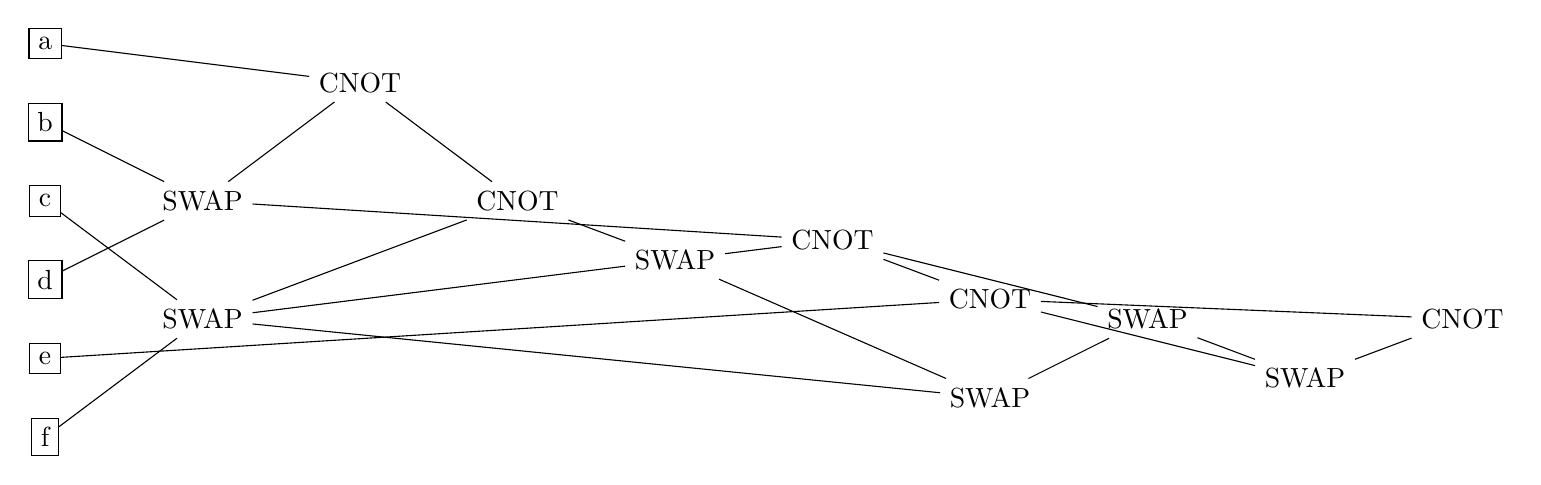
\begin{tikzpicture}
    
    \node [draw, rectangle] (a) at (0,5) {a};
    \node [draw, rectangle] (b) at (0,4) {b};
    \node [draw, rectangle] (c) at (0,3) {c};
    \node [draw, rectangle] (d) at (0,2) {d};
    \node [draw, rectangle] (e) at (0,1) {e};
    \node [draw, rectangle] (f) at (0,0) {f};
    
    \node (swap1) at (2,3) {SWAP};
    \node (swap2) at (2,1.5) {SWAP};
    \node (cnot1) at (4,4.5) {CNOT};
    \node (cnot2) at (6,3) {CNOT};
    \node (swap3) at (8,2.25) {SWAP};
    \node (cnot3) at (10,2.5) {CNOT};
    \node (cnot4) at (12,1.75) {CNOT};
    \node (swap4) at (12,0.5) {SWAP};
    \node (swap5) at (14,1.5) {SWAP};
    \node (swap6) at (16,0.75) {SWAP};
    \node (cnot5) at (18,1.5) {CNOT};
    
    \draw (b) -- (swap1);
    \draw (d) -- (swap1);
    
    \draw (c) -- (swap2);
    \draw (f) -- (swap2);
    
    \draw (a) -- (cnot1);
    \draw (swap1) -- (cnot1);
    
    \draw (cnot1) -- (cnot2);
    \draw (swap2) -- (cnot2);
    
    \draw (cnot2) -- (swap3);
    \draw (swap2) -- (swap3);
    
    \draw (swap1) -- (cnot3);
    \draw (swap3) -- (cnot3);
    
    \draw (cnot3) -- (cnot4);
    \draw (e) -- (cnot4);
    
    \draw (swap2) -- (swap4);
    \draw (swap3) -- (swap4);
    
    \draw (cnot3) -- (swap5);
    \draw (swap4) -- (swap5);
    
    \draw (cnot4) -- (swap6);
    \draw (swap5) -- (swap6);
    
    \draw (swap6) -- (cnot5);
    \draw (cnot4) -- (cnot5);
    
\end{tikzpicture}
}

Latency: \(1440 + 400 = 1840\) ns
\end{itemize}

\item {\bfseries\sffamily TODO} :B\(_{\text{noteNH}}\):
\label{sec:orgda82df7}
In this case, we can apply scheduling, indeed. The first result with an optimal routing and scheduling would be this one.

Note that the circuit complexity has grown and, thus, the amount of possible errors along the circuit.
Remember that Quantum gates are well known to be highly faulty.
\end{itemize}

\subsection*{Mapping example. Routing and re-scheduling}
\label{sec:org654f2fc}
\begin{itemize}
\item Example definition
\label{sec:org45eaba6}
\begin{itemize}
\item Example definition
\label{sec:orgf8559b5}
\begin{center}

Ex.: To map the Gray code generator Quantum Circuit for 6 \uline{physical} qubits in the SC-7.

\end{center}

\item Surface architecture
\label{sec:org9739756}

    \begin{center}
    \resizebox{\textwidth}{!}{%
    \begin{tikzpicture}[x=5mm,y=5mm]
% \tikzstyle{every node} = [circle, fill=gray!30]
% \node [green] at (0,0) {[circle, fill=gray!30]};
\draw node[fill=cyan,circle,minimum size=0.3cm] at (0,0) {};
% \node [cyan] at (10,0) {\textbullet};
\draw node[fill=cyan,circle,minimum size=0.3cm] at (10,0) {};
% \node [green] at (20,0) {\textbullet};
\draw node[fill=cyan,circle,minimum size=0.3cm] at (20,0) {};
% \node [red] at (5,5) {\textbullet};
\draw node[fill=cyan,circle,minimum size=0.3cm] at (5,5) {};
% \node [red] at (5,-5) {\textbullet};
\draw node[fill=cyan,circle,minimum size=0.3cm] at (5,-5) {};
% \node [red] at (15,5) {\textbullet};
\draw node[fill=cyan,circle,minimum size=0.3cm] at (15,5) {};
% \node [red] at (15,-5) {\textbullet};
\draw node[fill=cyan,circle,minimum size=0.3cm] at (15,-5) {};

\node [purple] at (2,0) {\textbf{c} $\to$ \textbf{2}};
\node [purple] at (12,0) {\textbf{d} $\to$ \textbf{3}};
\node [purple] at (22,0) {\textbf{e} $\to$ \textbf{4}};
\node [purple] at (7,5) {\textbf{a} $\to$ \textbf{0}};
\node [purple] at (7,-5) {\textbf{f} $\to$ \textbf{5}};
\node [purple] at (17,5) {\textbf{b} $\to$ \textbf{1}};
\node [purple] at (17,-5) {\textbf{6}};

% \draw[{Circle[red]}-Latex] (0,0) -- (2,0);
\draw[-Latex] (0.1, 0.4)  -- (4.6,4.9)   node [midway, above, sloped] {0};
\draw[-Latex] (4.8,4.7)   -- (0.3,0.2)  node [midway, below, sloped] {8};

\draw[-Latex] (5.4, 4.9)   -- (9.9,0.4)  node [midway, above, sloped] {1};
\draw[-Latex] (9.7,0.2) -- (5.2,4.7)   node [midway, below, sloped] {9};

\draw[-Latex] (10.1,0.4)  -- (14.6,4.9)  node [midway, above, sloped] {2};
\draw[-Latex] (14.8,4.7)  -- (10.3,0.2) node [midway, below, sloped] {10};

\draw[-Latex] (15.4, 4.9)  -- (19.9,0.4)  node [midway, above, sloped] {3};
\draw[-Latex] (19.7,0.2) -- (15.2,4.7)  node [midway, below, sloped] {11};

\draw[-Latex] (0.4,-0.1) -- (4.9,-4.6)  node [midway, above, sloped] {4};
\draw[-Latex] (4.7,-4.8) -- (0.2,-0.3)  node [midway, below, sloped] {12};

\draw[-Latex] (5.1, -4.6) -- (9.6,-0.1) node [midway, above, sloped] {5};
\draw[-Latex] (9.8, -0.3) -- (5.3, -4.8) node [midway, below, sloped] {13};

\draw[-Latex] (10.4,-0.1) -- (14.9,-4.6) node [midway, above, sloped] {6};
\draw[-Latex] (14.7,-4.8) -- (10.2,-0.3) node [midway, below, sloped] {14};

\draw[-Latex] (15.1,-4.6) -- (19.6,-0.1) node [midway, above, sloped] {7};
\draw[-Latex] (19.8,-0.3)  -- (15.3,-4.8) node [midway, below, sloped] {15};


\end{tikzpicture}
}
\end{center}


\item :B\(_{\text{ignoreheading}}\):
\label{sec:org78610e5}
\begin{itemize}
\item :B\(_{\text{structureenv}}\):
\label{sec:orgf66b419}
\begin{center}

\uline{Naive Approach}  

\medskip
\end{center}
\end{itemize}
\end{itemize}

\item :BMCOL:
\label{sec:org550eb64}



\item Gray Code Quantum Circuit
\label{sec:org0335086}
\begin{itemize}
\item :B\(_{\text{ignoreheading}}\):
\label{sec:orga84d96e}

\begin{center}
\resizebox{\textwidth}{!}{
    \Qcircuit @C=.5em @R=.7em {
 \lstick{a \to Q_0} & \qw & \qw & \qw & \qw & \targ & \qw & \qw & \qw & \qw & \qw & \qw & \qw & \qw & \qw & \qw & \qw & \qw & \qw\\
\lstick{b \to Q_1} & \qswap & \push{d} \qw & \qw & \qw & \qw & \qw & \qw & \qw & \ctrl{2} & \targ & \qw & \qw & \qw & \qw & \qswap & \push{f} \qw & \targ & \qw\\
\lstick{c \to Q_2} & \qw & \qw & \qswap & \push{f} \qw & \qw & \qw & \qw & \qw & \qw & \qw & \qswap & \push{b} \qw & \qw & \qw & \qw & \qw & \qw & \qw\\
\lstick{d \to Q_3} & \qswap \qwx[-2] & \push{b} \qw & \qw & \qw & \ctrl{-3} & \targ & \qswap & \push{c} \qw & \targ & \qw & \qw & \qw & \qswap & \push{f} \qw & \qswap \qwx[-2] & \push{d} \qw & \qw & \qw\\
\lstick{e \to Q_4} & \qw & \qw & \qw & \qw & \qw & \qw & \qw & \qw & \qw & \ctrl{-3} & \qw & \qw & \qw & \qw & \qw & \qw & \ctrl{-3} & \qw\\
\lstick{f \to Q_5} & \qw & \qw & \qswap \qwx[-3] & \push{c} \qw & \qw & \ctrl{-2} & \qswap \qwx[-2] & \push{b} \qw & \qw & \qw & \qswap \qwx[-3] & \push{f} \qw & \qswap \qwx[-2] & \push{c} \qw & \qw & \qw & \qw & \qw \gategroup{1}{2}{6}{5}{.7em}{--} \gategroup{1}{6}{6}{6}{.7em}{--} \gategroup{1}{7}{6}{7}{.7em}{--} \gategroup{1}{8}{6}{9}{.7em}{--} \gategroup{1}{10}{6}{10}{.7em}{--} \gategroup{1}{11}{6}{13}{.7em}{--} \gategroup{1}{14}{6}{15}{.7em}{--} \gategroup{1}{16}{6}{17}{.7em}{--} \gategroup{1}{18}{6}{18}{.7em}{--}
 }
}
\end{center}

\item :B\(_{\text{ignoreheading}}\):
\label{sec:org89ced38}
\begin{center}
$\Box$ \text{Cycle}
\end{center}

\item :B\(_{\text{ignoreheading}}\):
\label{sec:org04b6aee}
\resizebox{\textwidth}{!}{%
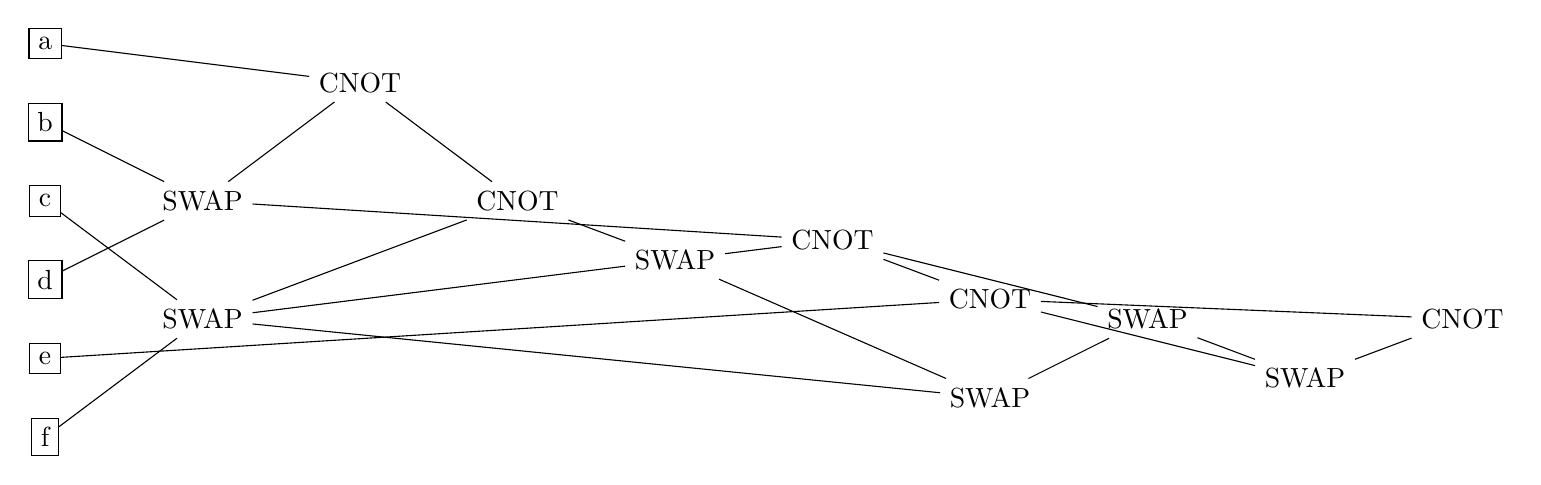
\begin{tikzpicture}
    
    \node [draw, rectangle] (a) at (0,5) {a};
    \node [draw, rectangle] (b) at (0,4) {b};
    \node [draw, rectangle] (c) at (0,3) {c};
    \node [draw, rectangle] (d) at (0,2) {d};
    \node [draw, rectangle] (e) at (0,1) {e};
    \node [draw, rectangle] (f) at (0,0) {f};
    
    \node (swap1) at (2,3) {SWAP};
    \node (swap2) at (2,1.5) {SWAP};
    \node (cnot1) at (4,4.5) {CNOT};
    \node (cnot2) at (6,3) {CNOT};
    \node (swap3) at (8,2.25) {SWAP};
    \node (cnot3) at (10,2.5) {CNOT};
    \node (cnot4) at (12,1.75) {CNOT};
    \node (swap4) at (12,0.5) {SWAP};
    \node (swap5) at (14,1.5) {SWAP};
    \node (swap6) at (16,0.75) {SWAP};
    \node (cnot5) at (18,1.5) {CNOT};
    
    \draw (b) -- (swap1);
    \draw (d) -- (swap1);
    
    \draw (c) -- (swap2);
    \draw (f) -- (swap2);
    
    \draw (a) -- (cnot1);
    \draw (swap1) -- (cnot1);
    
    \draw (cnot1) -- (cnot2);
    \draw (swap2) -- (cnot2);
    
    \draw (cnot2) -- (swap3);
    \draw (swap2) -- (swap3);
    
    \draw (swap1) -- (cnot3);
    \draw (swap3) -- (cnot3);
    
    \draw (cnot3) -- (cnot4);
    \draw (e) -- (cnot4);
    
    \draw (swap2) -- (swap4);
    \draw (swap3) -- (swap4);
    
    \draw (cnot3) -- (swap5);
    \draw (swap4) -- (swap5);
    
    \draw (cnot4) -- (swap6);
    \draw (swap5) -- (swap6);
    
    \draw (swap6) -- (cnot5);
    \draw (cnot4) -- (cnot5);
    
\end{tikzpicture}
}

Latency: 1520 ns
\end{itemize}


\item {\bfseries\sffamily TODO} :B\(_{\text{noteNH}}\):
\label{sec:org4e58ad8}
In this case, we can apply scheduling, indeed. The first result with an optimal routing and scheduling would be this one.

Note that the circuit complexity has grown. The mapping task is causing an obvious overhead.
\end{itemize}

\subsection*{Optimal approach vs Naive}
\label{sec:org1079284}

\begin{itemize}
\item Circuits
\label{sec:org39b073c}
\begin{itemize}
\item :BMCOL:
\label{sec:org35012ee}
      \begin{center}
\resizebox{.6\textwidth}{!}{
     \Qcircuit @C=1em @R=.7em {
     \lstick{a \to Q_0} & \targ & \qw & \qw & \qw & \qw & \qw\\
\lstick{b \to Q_2} & \ctrl{-1} & \targ & \qw & \qw & \qw & \qw\\
\lstick{c \to Q_5} & \qw & \ctrl{-1} & \targ & \qw & \qw & \qw\\
\lstick{d \to Q_3} & \qw & \qw & \ctrl{-1} & \targ & \qw & \qw\\
\lstick{e \to Q_1} & \qw & \qw & \qw & \ctrl{-1} & \targ & \qw\\
\lstick{f \to Q_4} & \qw & \qw & \qw & \qw & \ctrl{-1} & \qw
}
}
\end{center}


\item :BMCOL:
\label{sec:org44c5f58}

\begin{center}
\resizebox{\textwidth}{!}{
    \Qcircuit @C=.5em @R=.7em {
 \lstick{a \to Q_0} & \qw & \qw & \qw & \qw & \targ & \qw & \qw & \qw & \qw & \qw & \qw & \qw & \qw & \qw & \qw & \qw & \qw & \qw\\
\lstick{b \to Q_1} & \qswap & \push{d} \qw & \qw & \qw & \qw & \qw & \qw & \qw & \ctrl{2} & \targ & \qw & \qw & \qw & \qw & \qswap & \push{f} \qw & \targ & \qw\\
\lstick{c \to Q_2} & \qw & \qw & \qswap & \push{f} \qw & \qw & \qw & \qw & \qw & \qw & \qw & \qswap & \push{b} \qw & \qw & \qw & \qw & \qw & \qw & \qw\\
\lstick{d \to Q_3} & \qswap \qwx[-2] & \push{b} \qw & \qw & \qw & \ctrl{-3} & \targ & \qswap & \push{c} \qw & \targ & \qw & \qw & \qw & \qswap & \push{f} \qw & \qswap \qwx[-2] & \push{d} \qw & \qw & \qw\\
\lstick{e \to Q_4} & \qw & \qw & \qw & \qw & \qw & \qw & \qw & \qw & \qw & \ctrl{-3} & \qw & \qw & \qw & \qw & \qw & \qw & \ctrl{-3} & \qw\\
\lstick{f \to Q_5} & \qw & \qw & \qswap \qwx[-3] & \push{c} \qw & \qw & \ctrl{-2} & \qswap \qwx[-2] & \push{b} \qw & \qw & \qw & \qswap \qwx[-3] & \push{f} \qw & \qswap \qwx[-2] & \push{c} \qw & \qw & \qw & \qw & \qw \gategroup{1}{2}{6}{5}{.7em}{--} \gategroup{1}{6}{6}{6}{.7em}{--} \gategroup{1}{7}{6}{7}{.7em}{--} \gategroup{1}{8}{6}{9}{.7em}{--} \gategroup{1}{10}{6}{10}{.7em}{--} \gategroup{1}{11}{6}{13}{.7em}{--} \gategroup{1}{14}{6}{15}{.7em}{--} \gategroup{1}{16}{6}{17}{.7em}{--} \gategroup{1}{18}{6}{18}{.7em}{--}
 }
}
\end{center}
\end{itemize}

\item :B\(_{\text{ignoreheading}}\):
\label{sec:org1f6f1a3}
\begin{table}[htbp]
\centering
\begin{tabular}{lll}
 & Optimal approach & Naive apprach\\
\hline
\# operations & 5 & 11\\
latency & 400 ns & 1520 ns\\
\hline
\end{tabular}
\end{table}
\end{itemize}
\subsection*{What is the problem?}
\label{sec:org4d4699a}

\begin{itemize}
\item :BMCOL:
\label{sec:orge8fad42}
\begin{itemize}
\item :B\(_{\text{ignoreheading}}\):
\label{sec:org2466a67}
Error sources:

\begin{itemize}
\item Superconducting quantum gates are highly faulty
\item Decoherence (time)
\item Others
\end{itemize}

\item :B\(_{\text{ignoreheading}}\):
\label{sec:orgdf33a0d}
\vspace{.5cm}

\uline{No error correction} (despite we are working at \uline{physical} qubits level)
\end{itemize}


\item :BMCOL:
\label{sec:orgbff36cc}
\begin{itemize}
\item Windows error image
\label{sec:orgd853dd7}
\vspace{.5cm}

\begin{center}
\includegraphics[width=\textwidth]{figs/computer_error_windows.png}
\end{center}
\end{itemize}

\item :B\(_{\text{ignoreheading}}\):
\label{sec:org2c4df12}

\item Best Mapping
\label{sec:org02d2794}
Ideal mapping should not inject extra errors.

\item {\bfseries\sffamily TODO} :B\(_{\text{noteNH}}\):
\label{sec:org215369c}
What is the problem of this overhead?

There are a lot of error sources that affect the fidelity of a quantum algorithm result.
Each gate introduce the possibility of having errors, as well as the latency.
Time is the main problem in Quantum Computation.

We will assume that error correction is not possible, because we are working with qubits at its physical level.

So the problem in the mapping task is, which is the best mapping between all possibilities in order to introduce the less amount of errors as possible.
\end{itemize}

\subsection*{State of the Art of the mapping task}
\label{sec:org3d2ef7e}

\begin{itemize}
\item Index
\label{sec:orgf488010}
\begin{itemize}
\item What is the people doing?
\label{sec:org53f46ef}
\small

\begin{itemize}
\item Our group's mapping
\item "An Efficient Methodology for Mapping Quantum Circuits to the IBM QX Architectures"
\item "Qubit Allocation"
\item "Scheduling physical operations in a quantum information processor"
\item "Automated generation of layout and control for quantum circuits"
\item "Minimizing the latency of quantum circuits during mapping to the ion-trap circuit fabric"
\item "A quantum physical design  ow using ilp and graph drawing"
\item "An minlp model for scheduling and place- ment of quantum circuits with a heuristic solution approach"
\item "Determining the minimal number of swap gates for multi- dimensional nearest neighbor quantum circuits"
\item \ldots{}
\end{itemize}
\end{itemize}

\item Compare with what we want to do
\label{sec:orgac97c93}
\begin{table}[htbp]
\centering
\small
\begin{tabular}{p{3.5cm}|p{3cm}|p{3.5cm}}
 & Chip Architecture & Metric\\
\hline
 &  & \\
"An Efficient Methodology [\ldots{}]" & IBM QX & Cost \(\equiv\) \#operations\\
 &  & \\
"Qubit Allocation" & IBM QX & Cost \(\equiv\) \#operations\\
 &  & \\
Our group's mapping & QuTech SC-7/SC-17 & Latency\\
\end{tabular}
\end{table}

\vspace{1cm}

The other works metric is either the \uline{latency} or the \uline{\#operations}, never the "probability of success" of the quantum circuit.


\item {\bfseries\sffamily TODO} :B\(_{\text{noteNH}}\):
\label{sec:org3e2729f}
\begin{itemize}
\item :B\(_{\text{onlyenv}}\):
\label{sec:org94b331a}
And this problem is an important problem for the Quantum Computing community.
   Many works have tried to efficiently map physical quantum circuits on different qubit structures.


\item :B\(_{\text{onlyenv}}\):
\label{sec:org7310366}
\hline

All the works are using the latency or the number of operations as metric, or what is the same, they are looking for the best mapping optimizing in number of operations or latency.

It is fair to think that the longer the circuit, the worse the results.
But, what if even the best mapping is introducing that amount of errors that, in the end, the result has no sense?
No one is analyzing the success of the algorithms after the mapping task!
\end{itemize}
\end{itemize}

\subsection*{Other constraints}
\label{sec:org19a47a9}

\begin{itemize}
\item SC-17 topology
\label{sec:org96acfe9}
\begin{itemize}
\item Images
\label{sec:org47f8c7b}
\begin{center}
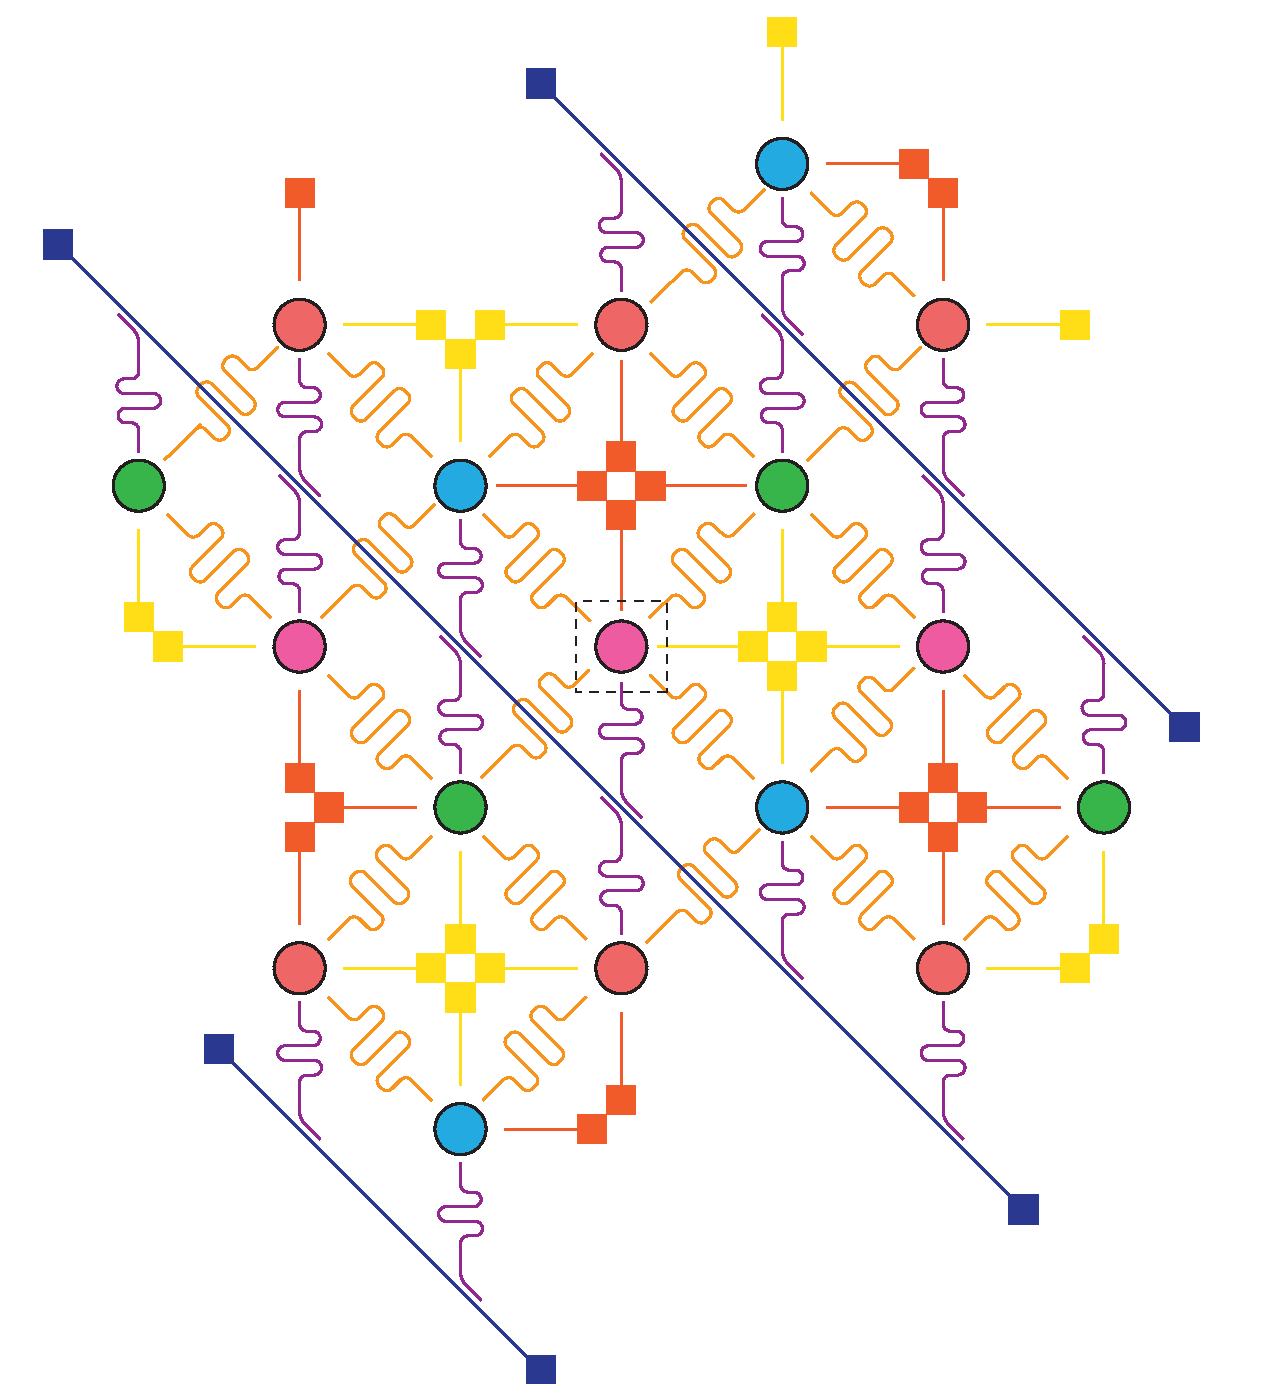
\includegraphics[width=.6\textwidth]{figs/sc-17.eps}
\end{center}

\item Images
\label{sec:orge25f548}
   
   \definecolor{qpink}{rgb}{0.91, 0.05, 0.57}
	      
     
     \begin{center}
     \resizebox{.75\textwidth}{!}{%

\begin{tikzpicture}[x=5mm,y=5mm]
\node [circle,fill=cyan,minimum size=10pt] at (20,10) {};
\node [circle,fill=green,minimum size=10pt] at (0,0) {};
\node [circle,fill=cyan,minimum size=10pt] at (10,0) {};
\node [circle,fill=green,minimum size=10pt] at (20,0) {};
\node [circle,fill=red,minimum size=10pt] at (5,5) {};
%\node [circle,fill=blue!50!red!50,minimum size=10pt] at (5,-5) {};
\node [circle,fill=qpink,minimum size=10pt] at (5,-5) {};
\node [circle,fill=red,minimum size=10pt] at (15,5) {};
\node [circle,fill=red,minimum size=10pt] at (25,5) {};
%\node [circle,fill=blue!50!red!50,minimum size=10pt] at (15,-5) {};
%\node [circle,fill=blue!50!red!50,minimum size=10pt] at (25,-5) {};
\node [circle,fill=qpink,minimum size=10pt] at (15,-5) {};
\node [circle,fill=qpink,minimum size=10pt] at (25,-5) {};
\node [circle,fill=green,minimum size=10pt] at (10,-10) {};
\node [circle,fill=cyan,minimum size=10pt] at (20,-10) {};
\node [circle,fill=green,minimum size=10pt] at (30,-10) {};
\node [circle,fill=red,minimum size=10pt] at (5,-15) {};
\node [circle,fill=red,minimum size=10pt] at (15,-15) {};
\node [circle,fill=red,minimum size=10pt] at (25,-15) {};
\node [circle,fill=cyan,minimum size=10pt] at (10,-20) {};

\node [purple] at (1,0) {\huge 4};
\node [purple] at (11,0) {\huge 5};
\node [purple] at (21,0) {\huge 6};
\node [purple] at (6,5) {\huge 1};
\node [purple] at (16,5) {\huge 2};
\node [purple] at (26,5) {\huge 3};
\node [purple] at (21,10) {\huge 0};
\node [purple] at (6,-5) {\huge 7};
\node [purple] at (16,-5) {\huge 8};
\node [purple] at (26,-5) {\huge 9};
\node [purple] at (11,-10) {\huge 10};
\node [purple] at (21,-10) {\huge 11};
\node [purple] at (31,-10) {\huge 12};
\node [purple] at (6,-15) {\huge 13};
\node [purple] at (16,-15) {\huge 14};
\node [purple] at (26,-15) {\huge 15};
\node [purple] at (11,-20) {\huge 16};

\draw (15,5) -- (20,10) node [midway, above, sloped] {};
\draw (20,10) -- (25,5) node [midway, above, sloped] {};
\draw (0,0) -- (5,5) node [midway, above, sloped] {};
\draw (5,5) -- (10,0)  node [midway, above, sloped] {};
\draw (10,0)  -- (15,5) node [midway, above, sloped] {};
\draw (15,5) -- (20,0) node [midway, above, sloped] {};
\draw (20,0) -- (25,5) node [midway, above, sloped] {};
\draw (20,0) -- (15, -5) node [midway, above, sloped] {};
\draw (15, -5) -- (10, 0) node [midway, above, sloped] {};
\draw (10, 0) -- (5, -5) node [midway, above, sloped] {};
\draw (5, -5) -- (0,0) node [midway, above, sloped] {};
\draw (20, 0) -- (25,-5) node [midway, above, sloped] {};
\draw (5, -5) -- (10,-10) node [midway, above, sloped] {};
\draw (10, -10) -- (15,-5) node [midway, above, sloped] {};
\draw (15, -5) -- (20,-10) node [midway, above, sloped] {};
\draw (20, -10) -- (25,-5) node [midway, above, sloped] {};
\draw (25, -5) -- (30,-10) node [midway, above, sloped] {};
\draw (5, -15) -- (10,-10) node [midway, above, sloped] {};
\draw (10, -10) -- (15,-15) node [midway, above, sloped] {};
\draw (15, -15) -- (20,-10) node [midway, above, sloped] {};
\draw (20, -10) -- (25,-15) node [midway, above, sloped] {};
\draw (25, -15) -- (30,-10) node [midway, above, sloped] {};
\draw (5, -15) -- (10,-20) node [midway, above, sloped] {};
\draw (10, -20) -- (15,-15) node [midway, above, sloped] {};

\draw (10,0) -- (15,5) -- (20, 0) --(15, -5) -- (10, 0) -- (5, -5) -- (0, 0);
\end{tikzpicture}

     }
     \end{center}
\end{itemize}


\item Constraints
\label{sec:org6238c18}
\begin{itemize}
\item :BMCOL:
\label{sec:org6761925}
Constraints:

\begin{itemize}
\item Frequencies constraint
\item Measurement constraint
\end{itemize}

\vspace{.5cm}

This constraints also affect the mapping task (mainly scheduling)

\item Table
\label{sec:org2f35707}
\definecolor{qpink}{rgb}{0.91, 0.05, 0.57}

\begin{center}
\begin{tabular}{ll}
 & \\
\hline
Freq. Group & Qubits\\
\hline
\cellcolor{red!25} QWG 0 & \cellcolor{red!25} 1, 2, 3, 13, 14, 15\\
\cellcolor{qpink!25} QWG 1 & \cellcolor{qpink!25} 7, 8, 9\\
\cellcolor{green!25} QWG 2 & \cellcolor{green!25} 4, 6, 10, 12\\
\cellcolor{cyan!25} QWG 3 & \cellcolor{cyan!25} 0, 5, 11, 16\\
\hline
\end{tabular}
\end{center}
\end{itemize}

\item {\bfseries\sffamily TODO} :B\(_{\text{noteNH}}\):
\label{sec:orgc5f82f6}
\uline{Frequencies constraint}

It is not possible to select or operate at the same time two different single-qubit gates over qubits in the same frequency set (same color).

\uline{Measurement constraint}

The measurement on a qubit cannot start when
 another qubit coupled to the same feedline is already being measured

This constraints are affecting mainly to the scheduling!
\end{itemize}

\section*{State of the art}
\label{sec:org7b5000c}

Quantum algorithms are meant to leverage the promising power of quantum computers \cite{coles18:quant_algor_implem_begin}.
Commonly described as quantum circuits, quantum algorithms are hardware agnostic.
Due to the variety of technologies that emerged with diverse specifications, there is a vast amount of literature on the algorithms -- high abstraction level --, neglecting hardware constraints.
From ion traps [? paper on ion traps] to superconducting qubits \cite{Barends_2014,Versluis_2017}, through quantum dots \cite{Hill_2015,Li_2018}, each layout has its own requirements and constraints.
Although all of them are arranged in a 2D -- planar -- structure, ion traps technologies are capable to connect the qubits in all-to-all networks while superconducting technologies connections form a grid shaped network where each qubit is connected to a maximum of four neighbors.
This grid behaviour establishes one of the main connectivity limitation in today's quantum chips, the NN constraint.
Also industry's superconducting chip layouts from IBM \cite{IBM_QX}, Google \cite{boixo16:charac_quant_suprem_near_term_devic} and Rigetti \cite{Sete_2016} follow this structural limitations.

As for the high abstraction level of the quantum algorithm, a link between the algorithms and the devices is required \cite{Fu_2016}.
As in classical computation, the algorithms should go through a compilation process in order to adapt them to the hosting device.
Certainly, the mapping procedure is an important element of this process based on three sub-tasks: scheduling, initial placement and routing; as we considered before.

There is a considerable amount of literature on the mapping task.
Initial works on this field \cite{Metodi_2006,Whitney_2007,Bahreini_2015} focused primarily on the definition of what they characterized as a \emph{scheduler} able to parallelize operations and add the required gates to route qubits.
They would consider general connectivity constraints as the NN one, common for most of the devices -- although the works were examining ion-traps as hardware implementations.
The proposed techniques by these works examine a dependency graph looking for the best way to organize qubits and operations.
The majority of the methods use latency as the metric to minimize, however some of them \cite{Farghadan_2017} would minimize in number of SWAP operations.
As it will be explained in the next section, to minimize in latency stands for time optimization while minimize in number of SWAP operations means to find the minimal number of operations required.
Following a similar reasoning as the first approaches, more complex solutions \cite{booth18:compar_integ_const_progr_tempor} have been published using Constraint Programming together with temporal planning, optimizing in latency as well.
Also, several publications \cite{Lye_2015,Wille_2016} outline only the routing sub-task using the number of SWAPS as the metric to minimize.

A recent review of the literature on the mapping topic focused on device specific mapping algorithms, with promising results.
In all the cases, taking into account the specific chip connectivity constrain.
IBM's chip have been gaining much attention due to the open online tools that make the chips accessible to everybody.
Various approaches to mapping algorithms for the IBM family of chips have been proposed \cite{zulehner17:effic_method_mappin_quant_circuit,Siraichi_2018,mckay18:qiskit_backen_specif_openq_openp_exper,Dueck_2018}.
Zulehner et. al \cite{zulehner17:effic_method_mappin_quant_circuit} developed a routing algorithm that optimizes in the number of SWAPs building a graph -- similarly to previous works --  and searching the best route in the chip layout with the A* algorithm.
Siraichi et. al \cite{Siraichi_2018} work defines a weighted dependence graph where the mapping algorithm is able to find a solution for all the mapping steps, initial placement, scheduling and routing.
Also, apart from the works related to the IBM devices, Rigetti's devices have been approached \cite{Venturelli_2018}.

In addition to the general connectivity limitations, quantum devices -- no matter which technology -- are error prone.
Quantum operations are faulty and qubits are not able to hold the desired state for long times, gradually rotating to another state -- the qubit decoheres.
For instance, in the case of superconducting technologies \cite{O_Brien_2017}, the chips bear with decoherence times of \(\approx 30 \mu s\) for qubit relaxation and \(\approx 60 \mu s\) for qubit dephase.
The error rates of single-qubit gates are less than 0.1\% taking \(> 20 ns\) to be executed, while two-qubit gates error rate is 0.6\% with times of \(40 ns\) and measurement error rates around 1\% with execution times of \(\sim 300 ns\) \cite{O_Brien_2017,Versluis_2017}.
This creates an undesirable environment to compute the most useful algorithms.
Therefore, in order to fight the errors generated by this behaviour, fault-tolerant (FT) and quantum error correction (QEC) mechanisms have been developed during the last years \cite{Nielsen_2009}.
These techniques force the quantum chips layout to arrange the qubits in a particular manner, constraining them even more.

Many attempts have been made \cite{Dousti_2014,Heckey_2015,hwang18:hierar_system_mappin_large_scale,murphy18:contr,Lao_2018} with the purpose of develop a FT mapping able to work at the logical -- qubit -- level.
However, due to the high complexity of the QEC techniques, quantum chips with large amounts of qubits are still theory.
More recent evidence \cite{Preskill_2018}, proposes the Noisy Intermediate-Scale Quantum (NISQ) devices as the next step for near future hardware with an amount of 50-100 qubits and without QEC or much simpler encodings.
Several studies, for instance \cite{tannu18:case_variab_aware_polic_nisq,paler18:nisq,paler18:influen_initial_qubit_placem_durin}, have been conducted on the mapping algorithms required for NISQ devices.
Also, the works on device specific solutions \cite{zulehner17:effic_method_mappin_quant_circuit,Siraichi_2018,mckay18:qiskit_backen_specif_openq_openp_exper,Dueck_2018,Venturelli_2018} described before, could be considered part of the NISQ works collection.
Although they do not approach the NISQ problem in general, it is true that the devices they tackle are NISQ devices, they have low number of qubits and high error rates.

Besides latency and the number of operations that serve to feedback the quality of a mapping algorithm, few studies have been published on quantum metrics.
Although widely investigated, there are not too many quantum metrics.
Fidelity has been addressed in order to characterize the error of a quantum circuit based on the qubits state \cite{Jozsa_1994,Nielsen_2009}.
And, recently, Quantum Volume has been defined to assert the capability of a quantum computer \cite{Moll_2018}.
In the next section and in \href{chapter-3.org}{Metrics} we offer an overview of the important metrics in this work.

\section*{Mapping metrics}
\label{sec:orgd805881}

As outlined in the state of the art, the literature considers mainly two metrics to optimize in their mapping algorithms, the added \textbf{latency} and the \textbf{number} of introduced \textbf{operations} after the mapping procedure.
The routing step from the mapping process introduces SWAP gates in the quantum circuit in order to move the qubits around in the layout.
And latency is the time required to run a quantum circuit in a given quantum device.
It depends on the chip cycle time and the \textbf{depth} of the circuit, that is the number of cycles the algorithm encloses.
Actually, most of the studies [REFERENCES] assert the latency in terms of circuit depth, avoiding the cycle time specification of any device.
E.g. in Fig. \ref{fig:latency_swaps_ex}, one can see how after the mapping process some SWAP operations have been added as well as the depth of the circuit or latency grows.
From five cycles depth in the original circuit to nine cycles.


\begin{figure}
    \centering

\subfigure[Gray encoder quantum circuit]{

\resizebox{0.3\textwidth}{!}{
   \Qcircuit @C=1em @R=.7em {
\lstick{a} & \targ & \qw & \qw & \qw & \qw & \qw\\
\lstick{b} & \ctrl{-1} & \targ & \qw & \qw & \qw & \qw\\
\lstick{c} & \qw & \ctrl{-1} & \targ & \qw & \qw & \qw\\
\lstick{d} & \qw & \qw & \ctrl{-1} & \targ & \qw & \qw\\
\lstick{e} & \qw & \qw & \qw & \ctrl{-1} & \targ & \qw\\
\lstick{f} & \qw & \qw & \qw & \qw & \ctrl{-1} & \qw
}
}

}
\label{fig:latency_swaps_ex_orig}

\subfigure[Mapped Gray encoder for the SC-7 chip. Each circuit part surrounded by a dashed line is a cycle]{

\resizebox{0.4\textwidth}{!}{
    \Qcircuit @C=.5em @R=.7em {
 \lstick{a \to Q_0} & \qw & \qw & \qw & \qw & \targ & \qw & \qw & \qw & \qw & \qw & \qw & \qw & \qw & \qw & \qw & \qw & \qw & \qw\\
\lstick{b \to Q_1} & \qswap & \push{d} \qw & \qw & \qw & \qw & \qw & \qw & \qw & \ctrl{2} & \targ & \qw & \qw & \qw & \qw & \qswap & \push{f} \qw & \targ & \qw\\
\lstick{c \to Q_2} & \qw & \qw & \qswap & \push{f} \qw & \qw & \qw & \qw & \qw & \qw & \qw & \qswap & \push{b} \qw & \qw & \qw & \qw & \qw & \qw & \qw\\
\lstick{d \to Q_3} & \qswap \qwx[-2] & \push{b} \qw & \qw & \qw & \ctrl{-3} & \targ & \qswap & \push{c} \qw & \targ & \qw & \qw & \qw & \qswap & \push{f} \qw & \qswap \qwx[-2] & \push{d} \qw & \qw & \qw\\
\lstick{e \to Q_4} & \qw & \qw & \qw & \qw & \qw & \qw & \qw & \qw & \qw & \ctrl{-3} & \qw & \qw & \qw & \qw & \qw & \qw & \ctrl{-3} & \qw\\
\lstick{f \to Q_5} & \qw & \qw & \qswap \qwx[-3] & \push{c} \qw & \qw & \ctrl{-2} & \qswap \qwx[-2] & \push{b} \qw & \qw & \qw & \qswap \qwx[-3] & \push{f} \qw & \qswap \qwx[-2] & \push{c} \qw & \qw & \qw & \qw & \qw \gategroup{1}{2}{6}{5}{.7em}{--} \gategroup{1}{6}{6}{6}{.7em}{--} \gategroup{1}{7}{6}{7}{.7em}{--} \gategroup{1}{8}{6}{9}{.7em}{--} \gategroup{1}{10}{6}{10}{.7em}{--} \gategroup{1}{11}{6}{13}{.7em}{--} \gategroup{1}{14}{6}{15}{.7em}{--} \gategroup{1}{16}{6}{17}{.7em}{--} \gategroup{1}{18}{6}{18}{.7em}{--}
 }
}

}
\label{fig:latency_swaps_ex_map}

\caption{Circuit mapping example}
\label{fig:latency_swaps_ex}
\end{figure}

The ideal mapping would be the one affecting the least as possible the original circuit or, what is the same, introducing the least amount of errors.
Clearly, both, latency and number of SWAPs, are direct effects of the mapping procedure that have an impact in the error increase as well.
To optimize in any of them stands on correct -- but not sufficient -- reasoning.
Latency optimization deems that the leading error source comes from the qubit lifetime.
And, indeed, time is a main issue in quantum computing.
Decoherence time is not only a maximum qubit lifetime, it is harder and harder to hold a quantum state for use times closer to the decoherence time.
On the other hand, to optimize in number of SWAPs stands on the intuition that the gate error is the preeminent error in a quantum device.
Although intuitively one can think that the more operations are in a circuit, the longer it will be; as seen in the [PROBLEM STATEMENT SECTION], the higher the number of operations does not necessarily mean the longer circuit depth.
Several operations can be run in parallel in the same cycle -- at the same time.
Actually, to minimize in latency is to maximize in parallelism.
Therefore, even though related, to optimize in one or the other holds different baselines.

Nonetheless, these metrics are not enough to assert how good the mapping process is.
They are related with the error rate increase but the relationship is not totally clear.
For instance, it could be the case that concatenation of errors introduced by contiguous gates would end up in a correction of the first error.
Or, that the busier the qubit is, the less affected by decoherence would be.
Then, one question arises.
What would be the best metric?
Definitely, the optimal solution would be to optimize directly in terms of the error rate.
But, in order to do that, a precise prediction of the error should be done and this is a hard computational task in quantum computing.

So that we could do a proper assessment of mapping algorithms, in our research we analyzed these two metrics amongst other different ones as fidelity, probability of success or quantum volume and their relationship with the error generated after the mapping.
We will define these metrics in the \href{chapter-3.org}{Metrics} section.
